\documentclass{beamer}

\usetheme{CambridgeUS}
\usecolortheme{seahorse}

\usepackage{geometry}

\usepackage{algorithm2e}
\usepackage{graphicx}
\usepackage{tabularx}
\usepackage{fourier}
\usepackage{hyperref}
\usepackage{multirow}
\usepackage{caption}
\usepackage{subcaption}
\usepackage{amsmath}
\usepackage{float}

\usepackage{xcolor}
\usepackage{listings}

\definecolor{mGreen}{rgb}{0,0.6,0}
\definecolor{mGray}{rgb}{0.5,0.5,0.5}
\definecolor{mPurple}{rgb}{0.58,0,0.82}
\definecolor{backgroundColour}{rgb}{0.95,0.95,0.92}

\lstdefinestyle{CStyle}{
	backgroundcolor=\color{backgroundColour},   
	commentstyle=\color{mGreen},
	keywordstyle=\color{magenta},
	numberstyle=\tiny\color{mGray},
	stringstyle=\color{mPurple},
	basicstyle=\footnotesize,
	breakatwhitespace=false,         
	breaklines=true,                 
	captionpos=b,                    
	keepspaces=true,                 
	numbers=left,                    
	numbersep=5pt,                  
	showspaces=false,                
	showstringspaces=false,
	showtabs=false,                  
	tabsize=2,
	language=C
}

\author{Alexane Boldo}

\institute{IMT Atlantique}

\title{Side-channel attacks on Ascon's S-box}

\date{2025}

\begin{document}
	\frame{\titlepage}
	
	\AtBeginSection[]
	{
		\begin{frame}
			\frametitle{Table of Contents}
			\tableofcontents[currentsection]
		\end{frame}
	}
	
	\begin{frame}
		\frametitle{Table of Contents}
		\tableofcontents
	\end{frame}
	
	\begin{frame}
		\frametitle{Introduction}
		\textbf{Side-Channel Attacks (SCA):} observation of computation time, power consumption, electromagnetic radiation, ... to discover a secret
		
		$\newline$
		
		\textbf{Goal:} Study the leaks from the Ascon S-box to theorize the best CPA attack
	\end{frame}
	
	
	\section{Correlation Power Analysis (CPA)}
	\subsection{Steps for the attack}
	\begin{frame}
		\frametitle{Steps for a CPA attack}
		
		\begin{columns}[T]
			\column{0.32\textwidth}
			\textbf{Campaign:}\\
			Choose:
			\begin{itemize}
				\item target $k$
				\item attack path $\mathcal{R}(k,O_S)=O_R$
			\end{itemize}
			Compute the algorithm multiple times to gain \textbf{traces}
			
			\column{0.32\textwidth}
			\textbf{Prediction:}\\
			Find a model for $\mathcal{R}$, $\mathcal{R}_m(k,O_S) = P_{m,k}$
			
			\column{0.32\textwidth}
			\textbf{Confrontation:}\\
			Choose a distinguisher for each hypothesis $k$, confronting $O_R$ and $P_{m,k}$\\
			Finds the best hypothesis $k_d$
		\end{columns}
	\end{frame}
	
	\subsection{Basic example on AES}
	\begin{frame}
		\frametitle{Example on AES}
		
		\begin{columns}[T]
			\column{0.32\textwidth}
			\textbf{Campaign:}\\
			\begin{itemize}
				\item $k = $ one byte of the secret key $K_0$
				\item $O_R = $ power consumption during the S-box
				\item $O_S = p$ one byte of the plaintext $T$
			\end{itemize}
			
			\column{0.32\textwidth}
			\textbf{Prediction:}\\
			$\mathcal{R}_m(k,p) = HW(S-box(p \oplus k))$
			\begin{figure}
				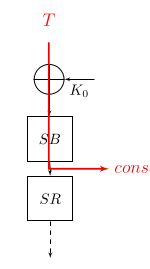
\includegraphics[width=0.5\textwidth]{attack_path_aes}
				\caption{Attack path on AES}
			\end{figure}
			
			\column{0.32\textwidth}
			\textbf{Confrontation:}\\
			Distinguisher: Pearson correlation
			\begin{figure}
				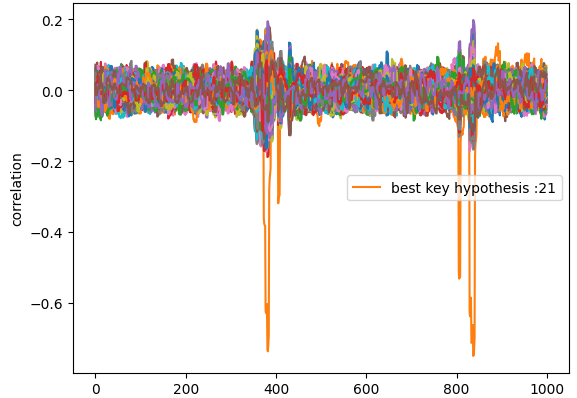
\includegraphics[width=\textwidth]{corr_aes}
				\caption{Correlation for each key hypothesis with the power consumption}
			\end{figure}
		\end{columns}
	\end{frame}
	
	
	\section{Ascon-AEAD}
	\subsection{Presentation}
	\begin{frame}
		\frametitle{What is Ascon?}
		\textbf{Authenticated Encryption with Associated Data (AEAD)}: encrypt, check authentication of content and associated data
		
		$\newline$
		
		NIST winner for lightweight cryptography
		
		$\newline$
		
		MonkeyDuplex based
	\end{frame}
	
	\subsection{The permutation}
	\begin{frame}
		\frametitle{Ascon's permutation(s)}
		$p = p_L \circ p_S \circ p_C$\\
		Intern permutation: $p^8$\\
		Extern permutation: $p^{12}$
		
		\begin{columns}[T]
			\column{0.32\textwidth}
			$$p_C$$
			$\newline$
				{\tiny 
				\begin{tabularx}{0.1\textwidth}{|*{8}{p{0.01cm}|}X}
					\cline{1-8}
					&&&&&&&&$S_0$\\
					\cline{1-8}
					&&&&&&&&$S_1$\\
					\cline{1-8}
					&&&&&&& \normalsize $\oplus$&$S_2$\\
					\cline{1-8}
					&&&&&&&&$S_3$\\
					\cline{1-8}
					&&&&&&&&$S_4$\\
					\cline{1-8}
				\end{tabularx}}
%				\caption{Constant-addition layer, each box representing a byte of one of the 64-bit words{}}
			
			\column{0.32\textwidth}
			$$p_S$$
			\begin{figure}
				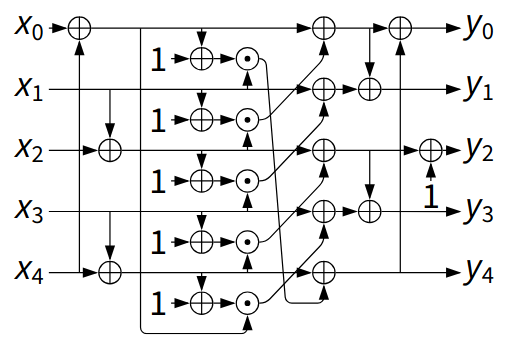
\includegraphics[scale=0.2]{circuit}
				\caption{Circuit to compute the S-box}
				\label{circuit_sbox}
			\end{figure}
			
			\column{0.32\textwidth}
			$$p_L$$
			\tiny
			\begin{gather*}
				\Sigma_0(S_0) = S_0 \oplus (S_0 >>> 19) \oplus (S_0 >>> 28)\\
				\Sigma_1(S_1) = S_1 \oplus (S_1 >>> 61) \oplus (S_1 >>> 39)\\
				\Sigma_2(S_2) = S_2 \oplus (S_2 >>> \;  1) \oplus (S_2 >>> \; 6)\\
				\Sigma_3(S_3) = S_3 \oplus (S_3 >>> 10) \oplus (S_3 >>> 17)\\
				\Sigma_4(S_4) = S_4 \oplus (S_4 >>> \; 7) \oplus (S_4 >>> 41)\\
			\end{gather*}
		\end{columns}
	\end{frame}
	
	\subsection{Encryption and decryption phases}
	\begin{frame}
		\frametitle{Encryption and decryption phases}	
		\begin{itemize}
			\item Initialization: state creation and modification
			$$S \leftarrow p^{a}( \underbrace{IV}_{S_0}||\underbrace{K}_{S_1,S_2}||\underbrace{n}_{S_3,S_4})$$
			$$S \leftarrow S \oplus 0^{192} || K$$
			\item Associated data process: updates the state using blocks of $r$-bits from $A=(A_1||..||A_s)$
			\item Plaintext/Ciphertext process: each block of the plaintext or ciphertext is included in the state
			\item Finalization: computes the tag thanks to the key and the state
		\end{itemize}	
	\end{frame}

	
	\section{Methodology}
	\subsection{Capture}
	\begin{frame}
		\frametitle{ChipWhisperer-Lite}
		\begin{columns}
			\column{0.45\textwidth}
			\begin{figure}[h]
				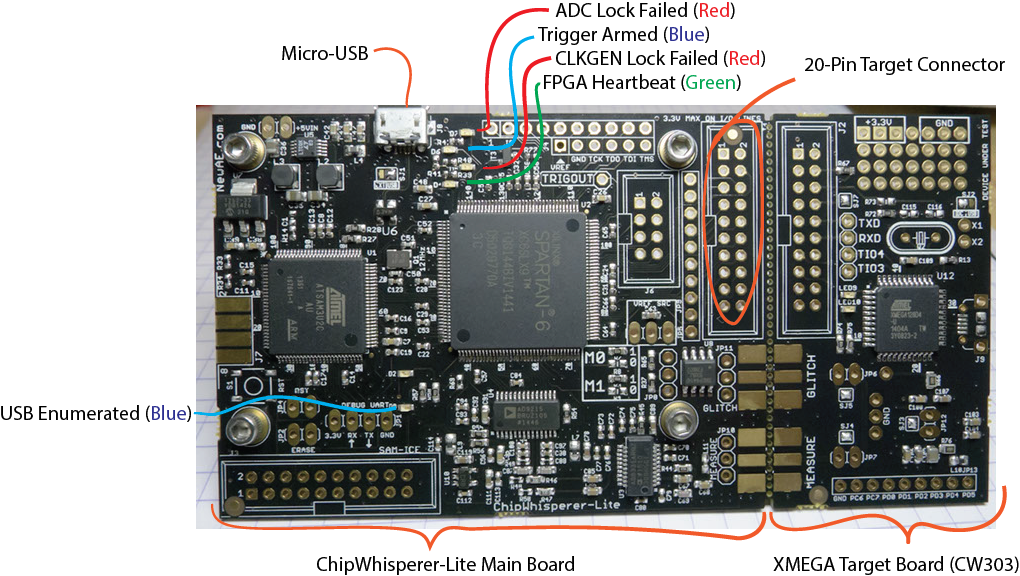
\includegraphics[width=\textwidth]{cwlite_basic1}
				\caption{ChipWhisperer Lite board}
				\label{fig:cw}
			\end{figure}
			
			\column{0.45\textwidth}
			\begin{itemize}
				\item Triggers around the S-box
				\item Traces with variable and fixed nonces  and keys captured
			\end{itemize}
		\end{columns}
	\end{frame}
	
	\subsection{Analysis}
	\begin{frame}
		\frametitle{Analyses done}
		\begin{itemize}
			\begin{columns}
				\column{0.55\textwidth}
				\item Finding the best theoretical attack path (HW vs value, vertical vs horizontal)
				\item Comparing distinguishers (Pearson correlation vs mutual information)
				\item Attack: finding the vertical output and deduct the key
				\column{0.4\textwidth}
				\begin{figure}[h]
					\centering
					\begin{tabular}{|c|c|}
						\hline
						$(n_0^j,n_1^j,IV^j)$&$S_4^j$\\
						\hline\hline
						$(0,0,0)$&$k_0^j$\\
						\hline
						$(0,0,1)$&$0$\\
						\hline
						$(0,1,0)$&$1$\\
						\hline
						$(0,1,1)$&$1 \oplus k_0^j$\\
						\hline
						$(1,0,0)$&$1 \oplus k_0^j$\\
						\hline
						$(1,0,1)$&$1$\\
						\hline
						$(1,1,0)$&$0$\\
						\hline
						$(1,1,1)$&$k_0^j$\\
						\hline
					\end{tabular}
					\caption{Link between $k_0^j$ and $S_4^j$ depending on $IV$ and $N$}
					\label{link_k_s4}
				\end{figure}
			\end{columns}
		\end{itemize}
	\end{frame}
	
	
	\section{Results}
	\begin{frame}
		\frametitle{Results vertical vs horizontal}
		\begin{figure}[h]
			\centering
			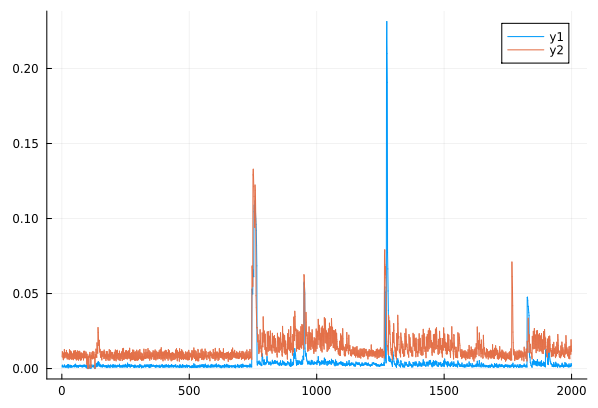
\includegraphics[scale=0.3]{h_and_v_one_byte}
			\caption{Mutual information for the horizontal and the vertical value}
			\label{hvval}
		\end{figure}
	\end{frame}
	
	\begin{frame}
		\frametitle{Results HW vs value}
		\begin{figure}
			\centering
			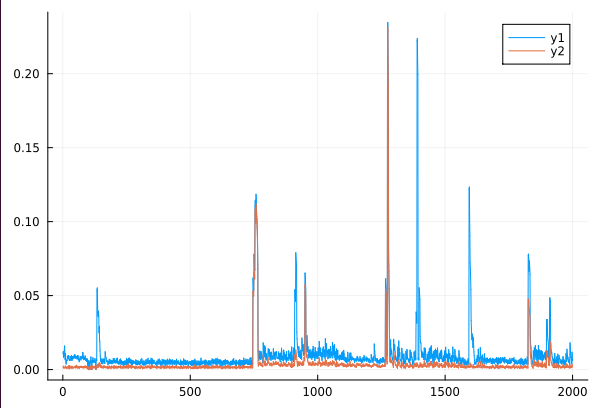
\includegraphics[scale=0.3]{vertical_one_bit}
			\caption{Mutual information between power consumption and Hamming weight of the concatenation of the first bit of each of the word of $S$ and its value}
			\label{vHW}
		\end{figure}
	\end{frame}
	
	\begin{frame}
		\frametitle{Results distinguisher}
		\begin{figure}
			\centering
			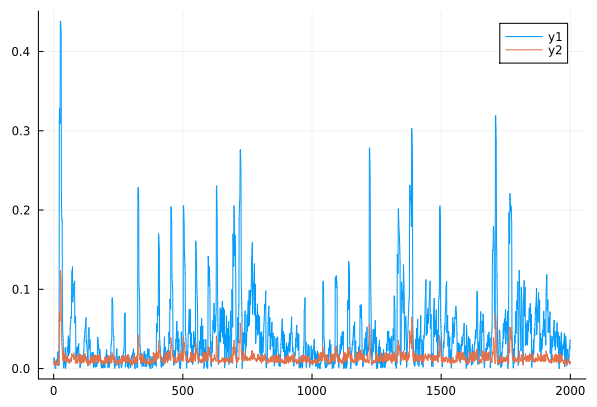
\includegraphics[scale=0.3]{corr_vs_MI_hHW}
			\caption{Mutual information and absolute Pearson correlation for a horizontal attack on the reference implementation}
			\label{corvsMI}
		\end{figure}
	\end{frame}
	
	\begin{frame}
		\frametitle{Results attack}
		\begin{figure}[h]
			\centering
			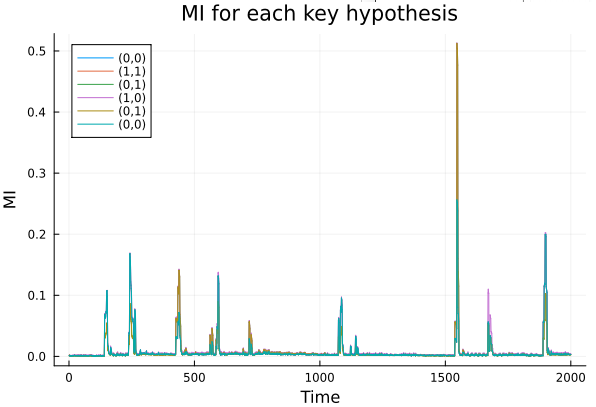
\includegraphics[scale=0.3]{nonces_alea}
			\caption{Mutual information between the Hamming weight of the outputs and the power consumption, for each of the possible outputs for the first nonce}
			\label{all_alea}
		\end{figure}
	\end{frame}
	
	\section{Conclusion}
	\begin{frame}
		\frametitle{Conclusion}
		\begin{itemize}
			\item Apparent weaknesses
			\item Unsuccessful attempts
			\item Leads to follow: belief propagation
		\end{itemize}
	\end{frame}

\end{document}